%\documentclass[12pt]{scrbook}
%
%\usepackage{tikz}
%\usepackage{minted}
%\usetikzlibrary{decorations.pathreplacing,arrows}
%\usetikzlibrary{arrows,decorations.pathmorphing,backgrounds,positioning,fit,petri}
%
%\usepackage{fullpage}
%\usepackage{subfigure}
%\begin{document}
%
%
%Lorem Ipsum is simply dummy text of the printing and typesetting industry. Lorem Ipsum has been the industry's standard dummy text ever since the 1500s, when an unknown printer took a galley of type and scrambled it to make a type specimen book. It has survived not only five centuries, but also the leap into electronic typesetting, remaining essentially unchanged. It was popularised in the 1960s with the release of Letraset sheets containing Lorem Ipsum passages, and more recently with desktop publishing software like Aldus PageMaker including versions of Lorem Ipsum.
%




\begin{figure}
\centering

\subfigure[First (and only) iteration.  In this partitioning, 9 is the pivot.
The index variable $i$ is incremented to 34 while $j$ decrements 
to match.  34 is swapped with itself.  After this iteration, the second
condition applies and the pivot is swapped with $a_{i-1} = 4$]{

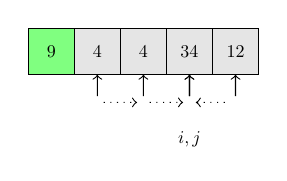
\begin{tikzpicture}[scale=.65,transform shape]

%\tikzset{>=stealth',shorten <=.2cm,>=stealth',shorten >=.2cm}
% size of each node
\def\sz{9mm}
% node style definition
\tikzstyle{block} = [
	draw, fill=black!10, rectangle,
	minimum height=\sz, minimum width=\sz ];
\tikzstyle{plain} = [draw=none,fill=none];

\node[block,fill=green!50] (a0) at (0*\sz,0) { 9 };
\node[block] (a1) at (1*\sz,0) { 4 };
\node[block] (a2) at (2*\sz,0) { 4 };
\node[block] (a3) at (3*\sz,0) { 34 };
\node[block] (a4) at (4*\sz,0) { 12 };

\node[below of=a1] (c1) {};
\draw[->] (c1) -- (a1);
\node[below of=a2] (c2) {};
\draw[->] (c2) -- (a2);
\node[below of=a3] (c3) {};
\draw[->] (c3) -- (a3);
\draw[->,dotted] (c1) -- (c2);
\draw[->,dotted] (c2) -- (c3);

\node[below of=a3] (d3) {};
\draw[->] (d3) -- (a3);
\node[below of=a4] (d4) {};
\draw[->] (d4) -- (a4);

\draw[<-,dotted] (d3) -- (d4);
\node[below of=c3,above] {$i,j$};


%\draw [decorate,decoration={brace,mirror,amplitude=5pt},xshift=-4pt,yshift=0pt] ([xshift=0cm,yshift=0cm]c1.south) -- ([xshift=0cm,yshift=0cm]c4.south) node [black,midway,yshift=-0.75cm] {$i$};

%\draw[<->,>=stealth',shorten <=.2cm,>=stealth',shorten >=.2cm] (a1.south) to [bend right] node[pos=.5,below] {swap} (a4.south);

%\draw[<->] (a4.south) to [in=270,out=270,looseness=1] node[pos=.5,below] {swap} (a8.south);

\end{tikzpicture}~~~~~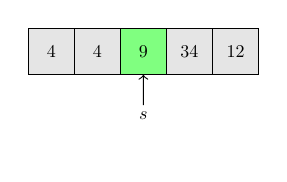
\begin{tikzpicture}[scale=.65,transform shape]

\def\sz{9mm}
\tikzstyle{block} = [
	draw, fill=black!10, rectangle,
	minimum height=\sz, minimum width=\sz ];
\tikzstyle{plain} = [draw=none,fill=none];
\draw[white] (0,0) rectangle (1, -2);

\node[block] (a0) at (0*\sz,0) { 4 };
\node[block] (a1) at (1*\sz,0) { 4 };
\node[block,fill=green!50] (a2) at (2*\sz,0) { 9 };
\node[block] (a3) at (3*\sz,0) { 34 };
\node[block] (a4) at (4*\sz,0) { 12 };

\node[below of=a2,node distance=1.25cm] (c2) {$s$};
\draw[->] (c2) -- (a2);

\end{tikzpicture}

}

\caption[Partitioning Example 3]{Example execution of the \textsc{Partition}
subroutine in Quick Sort on the second recursive call on the right partition.  
A total of 5 comparisons are made, 6 if you count the last swap outside the 
while loop.  The partition returns $s$ as the pivot position.}
\label{figure:partitionExample3}

\end{figure}


%\end{document}

